\documentclass[conference]{IEEEtran}
\IEEEoverridecommandlockouts
% The preceding line is only needed to identify funding in the first footnote. If that is unneeded, please comment it out.
\usepackage{cite}
\usepackage{amsmath,amssymb,amsfonts}
\usepackage{algorithmic}
\usepackage{graphicx}
\usepackage{textcomp}
\usepackage{xcolor}
\usepackage{float}
\usepackage{minted}
\usepackage{cuted}%%\stripsep-3pt

\def\BibTeX{{\rm B\kern-.05em{\sc i\kern-.025em b}\kern-.08em
    T\kern-.1667em\lower.7ex\hbox{E}\kern-.125emX}}
\begin{document}

\title{Github Data Analysis\\
{\small Wide Project Proposal}
}

\author{
\IEEEauthorblockN{YUAN Yingzhe}
\IEEEauthorblockA{\textit{Computer Science and Enigeering} \\
\textit{HKUST}\\
Hongkong, China }
\and
\IEEEauthorblockN{GUO Jiong}
\IEEEauthorblockA{\textit{Computer Science and Enigeering} \\
\textit{HKUST}\\
Hongkong, China}
}

\maketitle

% \begin{abstract}
%     Github is an open source platform for developers to share their codes and collaborate with others. In this project, we will use spark to construct a real-time processing framework, which aims at handling massive activity records and analyze data to find out patterns of users, repositories and languages. 
% \end{abstract}

% \begin{IEEEkeywords}
% Github, Spark, Data Analysis, Data Mining
% \end{IEEEkeywords}


\section{Introduction}

Github is an open source platform for developers to share their codes and collaborate with others. In this project, we will use spark to construct a real-time processing framework, which aims at handling massive activity records and analyze data to find out patterns of users, repositories and languages. 

\section{Dataset}

All the data we will use in this project are from Github. There is not an existing complete dataset to get enough well-structured data for our project, so we need to collect data and preprocess by ourselves. In this section, we will illustrate why we choose Github's data and what the data sources are.

\subsection{Why Github}
Github is the largest developer community and the largest platform for developers to share their codes and collaborate with others in the world. By analyzing the data from Github, we can get some insights about the development of open source projects, the development of programming languages, and the development of the developer community.



\subsection{Source I: Open API}
Github provides a series of open API for developers to access most of the informations on Github. This 'Github REST API\cite{ghapi}' is mainly used for creating integrations, retrieve data, and automate workflows, but we can use it to query specific data needed for our project.

There are mainly two main areas of data:

\begin{itemize}
    \item \textbf{Users:} Basic open informations of user, such as id, name, email, following users, repositories owned, etc.
    \item \textbf{repositories:} Basic information of public repositories, such as id, name, owner, description, stars etc.
\end{itemize}

We will provide some examples results of API query in Appendix\ref{a-ghrest}.

There are limits of current official REST API:
\begin{itemize}
    \item Some need authentication, which means we need to provide a valid token to access the data.
    \item Some API cannot be called too frequently, which means we need to wait for a while before we can call it again.
    \item Most of API need an \textbf{\textit{id}} as its query parameter, so we need to get the id first before we can query the data, which means we need to construct a massive id list.
\end{itemize}

After considering the above limitations, we decide to use the Github Archive\cite{gha} as our main data source and use the REST API to get some additional data or search some specific content.


\subsection{Source II: Github Archive}

\textit{GH Archive\cite{gha} is a project to record the public GitHub timeline, archive it, and make it easily accessible for further analysis.} In fact, it also based on Github's Open API, while only use the \textbf{activity} API:



\begin{minted}[breaklines,breakautoindent,mathescape,linenos,numbersep=1pt,frame=lines,framesep=2mm,fontsize=\footnotesize,baselinestretch =1,style=emacs]{python}
    https://api.github.com/events
\end{minted}


\textbf{GH Archive} will crawl github's activity data in real time and sort them as json file in order of when they occurred. Activity archives are available starting from 2011-02-12, and are updated amost half day, so the total size of data is \textbf{TB} level. 

Considering too large size of the data and the the earlist data using a different format, we will only use the latest part of them. In fact, the current amount data of data in an hour is about 700MB, so the latest data is surely enough for our project. The corresponding compression packages with specific time can be downloaded easily, and the minimal time interval of packages is one hour. 

\begin{figure}[H]
    \centering
    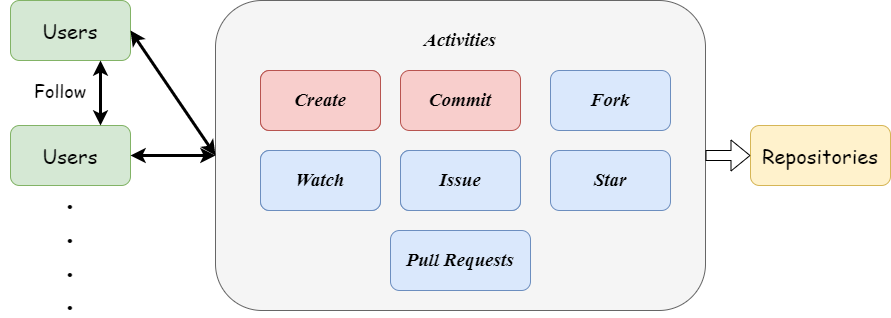
\includegraphics[width=0.45\textwidth]{./pic/github.png}
    \caption{This figure shows relation between user and repository and basic activities.}
    \label{fig:github}
\end{figure}


The archieved activity data contains almost all 20+ event types provided by Github, which ranges from new commits and fork events, to adding members to a project. We will only pay attention to some key event type, such as \textit{commit}, \textit{create}, etc.

We will give some example of the data format in Appendix\ref{a-gha}.


\subsection{Summary}
Based on almost all activity record, Github's Open API can help us to get almost all related information. For example, from \textbf{GH archive}, we know user a push a commit at 12:00 in repository A, then we can get almost all details of a and A by calling Github's API.








\section{Task}

Github has provided some basic data aggregation for user to explore. For example, in \textbf{\textit{Trending\cite{ghtrending}}}, Github shows the most popular repositories in the specific time range, language and spoken language. In \textbf{\textit{Topics\cite{ghtopics}}}, Github shows repositories' topics according to tags of repositories. However, these data analysis are very basic and not wide to cover most of the information in Github.

In this project, we will use spark to construct a real-time processing framework, which aims at handling massive activity records and analyze data to give a more comprehensive analysis of Github.

There are main tasks in this project:

\subsection{Data Preprocess}

\begin{enumerate}
    \item \textbf{Collect} data. Crawl Github Archive\cite{gha} and use Github API\cite{ghapi} to jointly query more detailed information about activities according to indices in Github Archive. Though Github Archive update several times a day, we will simulate it to a real-time stream to process data in real-time. 
    \item \textbf{Preprocess} data by Spark. For complete each json record, split it into several parts, filter useful parts and store them in different tables.
    \item Data \textbf{Persistence}. Design different schema and construct key meta tables to store necessary information, statistics result or some data not easily obtained directly.
\end{enumerate}

\subsection{Data Analysis}

\begin{enumerate}
    \item \textbf{Statistics}. We wiil try to construct a dashboard to show some basic statistics of Github, such as the repository with the highest frequency of commits, the most frequently commits time period, etc.
\end{enumerate}


\subsection{Data Visualization}
\begin{enumerate}
    \item \textbf{Dashboard}. We will try to construct a dashboard to watch the process of data process and show the results of data analysis by deploying a webpage.
    \item \textbf{Interaction}. We will try to make the dashboard interactive, such as users can choose the time range of data to analyze, or choose the language to analyze, etc. Results of corresponding process not only comes from persistant database, but also from real-time stream produced by Spark.
\end{enumerate}








\section{Technologies}

The technologies we will use in this project can be divided into three parts roughly: big data process, data visualization and environment deploy. Some of them are not sure if they will be used. 

The details are as followed:

% \begin{strip}
    \begin{figure}[H]
        \centering
        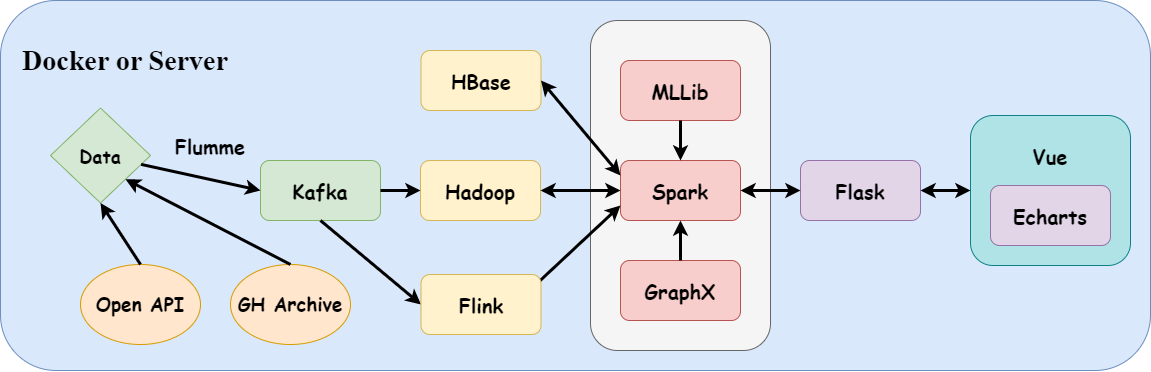
\includegraphics[width=0.53\textwidth]{./pic/dataflow.png}
        \caption{This picture show the rough technologies based on Dataflow.}
        \label{fig:dataflow}
    \end{figure}
% \end{strip}


\subsection{Big Data Process}

\begin{enumerate}
    \item \textbf{Spark}. As a computing engine, it will perform most of the data processing tasks.
    \item \textbf{Flumme} As a data collector, it will collect data from Github Archive and Github API.
    \item \textbf{Kafka}. As a message queue, it will simulate the real-time stream of Github Archive.
    \item \textbf{HDFS}. As a distributed file system, it will store the intermediate data as file or some persistant data.
    \item \textbf{Hive}. As a data warehouse, it will store the persistant data in tables.
    \item \textbf{Flink}. As a stream processing engine, it will process the real-time stream.
    \item \textbf{MLLib}. As a machine learning library, it will be used to extract features from data and finish some basic prediction tasks.
    \item \textbf{GraphX}. As a graph processing library, it will be used to construct a social graph.
    \item \textbf{HBase}. As a NoSQL database, it will be used to store some persistant data.
    \item \textbf{SparkNLP}. As a open-source library, it will perform the complicated NLP tasks. We will explore how to integrate it with Spark, because it's not an official library of Apache.
\end{enumerate}


\subsection{Data Visualization}

\begin{enumerate}
    \item \textbf{Vue}. As a front-end framework, it will be used to construct the basic framework of dashboard.
    \item \textbf{Echarts}. As a data visualization library, it will be used to visualize the results of data analysis.
\end{enumerate}

\subsection{Environment Deploy}

\begin{enumerate}
    \item \textbf{Docker}. Though the final application will be deployed on several cloud clusters. we may consider to deploy test environment on a powerful single machine locally by using Docker. By self-define images, it will help us construct the whole system easily and quickly.
    \item \textbf{Kubernetes}. As a container orchestration engine, it will be used to manage the containers. This will be used as a backup to set up the test system.
\end{enumerate}



\section{Summary}

Based on Github's activity data, we will use Spark and corresponding tools to construct a real-time processing framework, which will be deployed on a cloud cluster. We will show more comprehensive analysis of Github by using this framework.



% \section*{Acknowledgment}

% The contribution of our team members are as follows:



\begin{thebibliography}{00}
\bibitem{gha}https://www.gharchive.org/
\bibitem{ghapi}https://docs.github.com/en/rest?apiVersion=2022-11-28
\bibitem{ghtrending}https://github.com/trending
\bibitem{ghtopics}https://github.com/topics
\end{thebibliography}

\appendices

\section{Github REST API Example}
\label{a-ghrest}

There are some API's calling examples.


\subsection{Get All Followers of a User}

\begin{minted}[breaklines,breakautoindent,mathescape,linenos,numbersep=1pt,frame=lines,framesep=2mm,fontsize=\footnotesize,baselinestretch =1,style=emacs]{python}
    https://api.github.com/users/mateiz/followers
\end{minted}


\begin{minted}[breaklines,breakautoindent,mathescape,linenos,numbersep=1pt,frame=lines,framesep=2mm,fontsize=\footnotesize,baselinestretch =1,style=emacs]{json}
    [
        {
            "login": "bennettandrews",
            "id": 1143,
            "node_id": "MDQ6VXNlcjExNDM=",
            "avatar_url": "https://avatars.githubusercontent.com/u/1143?v=4",
            "gravatar_id": "",
            "url": "https://api.github.com/users/bennettandrews",
            "html_url": "https://github.com/bennettandrews",
            ...
        },
        ...
    ]
\end{minted}


\subsection{Get Repository's Detailed Information}

\begin{minted}[breaklines,breakautoindent,mathescape,linenos,numbersep=1pt,frame=lines,framesep=2mm,fontsize=\footnotesize,baselinestretch =1,style=emacs]{python}
    https://api.github.com/repos/apache/spark
\end{minted}


\begin{minted}[breaklines,breakautoindent,mathescape,linenos,numbersep=1pt,frame=lines,framesep=2mm,fontsize=\footnotesize,baselinestretch =1,style=emacs]{json}
    {
        "id": 17165658,
        "node_id": "MDEwOlJlcG9zaXRvcnkxNzE2NTY1OA==",
        "name": "spark",
        "full_name": "apache/spark",
        "private": false,
        "owner": {
            "login": "apache",
            "id": 47359,
            ...
        }
        ...
    }
\end{minted}



\subsection{Get All Commits of a Repository}

\begin{minted}[breaklines,breakautoindent,mathescape,linenos,numbersep=1pt,frame=lines,framesep=2mm,fontsize=\footnotesize,baselinestretch =1,style=emacs]{python}
    https://api.github.com/repos/apache/spark/commits
\end{minted}


\begin{minted}[breaklines,breakautoindent,mathescape,linenos,numbersep=1pt,frame=lines,framesep=2mm,fontsize=\footnotesize,baselinestretch =1,style=emacs]{json}
    [
        {
            "sha": "0fde146e8676ab9a4aeafebb1684eb7a44660524",

            "commit": {
                "author": {
                    "name": "Juliusz Sompolski",
                    "email": "julek@databricks.com",
                    "date": "2023-03-24T01:56:26Z"
                },
                "committer": {
                    "name": "Hyukjin Kwon",
                    "email": "gurwls223@apache.org",
                    "date": "2023-03-24T01:56:26Z"
                },
                "message": "...",
                "tree": {
                    "sha": "308faa10a134402eb4e0796c54b4e4dd000fc7dc"
                },
                ...
            },
            "author": {
                "login": "juliuszsompolski",
                "id": 25019163,
                "node_id": "MDQ6VXNlcjI1MDE5MTYz",
                ...
            },
            "committer": {
                "login": "HyukjinKwon",
                "id": 6477701,
                ...
            },
            "parents": [{}]
        },
        ...
    ]
\end{minted}




\section{GH Archive}
\label{a-gha}

One single json record from the GH Archive.

\begin{minted}[breaklines,breakautoindent,mathescape,linenos,numbersep=1pt,frame=lines,framesep=2mm,fontsize=\footnotesize,baselinestretch =1,style=emacs]{json}
    [
        {
            "id": "2489651051",
            "type": "PushEvent",
            "actor": {
                "id": 3854017,
                "login": "rspt",
                "gravatar_id": "",
                "url": "https://api.github.com/users/rspt",
                "avatar_url": "https://avatars.githubusercontent.com/u/3854017?"
            },
            "repo": {
                "id": 28671719,
                "name": "rspt/rspt-theme",
                "url": "https://api.github.com/repos/rspt/rspt-theme"
            },
            "payload": {
                "push_id": 536863970,
                "size": 1,
                "distinct_size": 1,
                "ref": "refs/heads/master",
                "head": "6b089eb4a43f728f0a594388092f480f2ecacfcd",
                "before": "437c03652caa0bc4a7554b18d5c0a394c2f3d326",
                "commits": [
                    {
                        "sha": "6b089eb4a43f728f0a594388092f480f2ecacfcd",
                        "author": {
                            "email": "5c682c2d1ec4073e277f9ba9f4bdf07e5794dabe@rspt.ch",
                            "name": "rspt"
                        },
                        "message": "Fix main header height on mobile",
                        "distinct": true,
                        "url": "https://api.github.com/repos/rspt/rspt-theme/commits/6b089eb4a43f728f0a594388092f480f2ecacfcd"
                    }
                ]
            },
            "public": true,
            "created_at": "2015-01-01T15:00:01Z"
        },
        ...
    ]
\end{minted}




\end{document}
